\documentclass[%
reprint,nofootinbib,
amsmath,amssymb,
aps,
]{revtex4-1}
\usepackage{graphicx}% Include figure files
\usepackage{dcolumn}% Align table columns on decimal point
\usepackage{bm}% bold math
\usepackage[utf8]{inputenc}
\usepackage{listings}
\usepackage{amsmath}
\usepackage{physics}
\usepackage{booktabs}
\usepackage{float}
\usepackage[bottom]{footmisc}
\usepackage{scrextend}
\bgroup
\def\arraystretch{1.3}
\newcommand{\HRule}{\rule{\textwidth}{0.5mm}}
\makeatletter
\newcommand*{\rom}[1]{\expandafter\@slowromancap\romannumeral #1@}
\makeatother

\begin{document}
\onecolumngrid

\begin{center}
	\large\textbf{The Ising Model\\ \small{Studies of phase transitions in magnetic systems}}
\end{center}
\vspace{5mm}

\begin{center}
	\small{$^1$ Oline A. Ranum}\\
\end{center}

\begin{center}
	\small{$^1$ University of Oslo, Institute of physics, 
		olinear@student.matnat.uio.no}
\end{center}

\begin{center}
	\textit{\today}
\end{center}
\vspace{7mm}
\noindent 
\HRule \vspace{2mm}\\
The main objective of this paper is to simulate the evolution of a lattice  spin system by employing the Ising model. The evolution process is propagated using a Monte Carlo Metropolis procedure. Finite lattices of size $L = \{2, 20, 40, 60, 80, 100\}$ are considered for temperatures ranging from $T = 1.0$ $k_bT/J$ to $T = 2.5$  $k_bT/J$, for $N = 10^i$ with $i = \{4, 5, 6, 7, 8\}$  Monte Carlo iteration. Estimates were made of $\expval{E}$, $\expval{E^2}$, $\expval{M}$, $\expval{M^2}$, $\expval{\abs{M}}$, the magnetic susceptibility $\chi$ and the heat capacity $C_V$. It was found that  $N = 10^7$ iterations was sufficient to yield a good approximation to the exact results for $L = 2$, with an accuracy of minimum three leading digits for all estimated values. The equilibration time of the system was found to be $
t_{eq} \approx 2.5\times10^5 \hspace{3mm}[N_{sweeps}]$ for  $T = 1.0$ $k_bT/J$   and $t_{eq} \approx 2.5\times10^4 \hspace{3mm}[N_{sweeps}]$ for $T = 2.4$ $k_bT/J$. The equilibration time appears to decrease in response to increasing the temperature, consistent with a higher number of cycles being accepted at each Monte Carlo sweep for $T =2.4 $ $k_bT/J$ than for $T = 1.0$ $k_bT/J$. Plots of the energy distribution is presented as a function of T, where an increase in temperature indicated access to a larger number of microstates. The results are consistent with the basics of thermodynamics. The final section of the paper looks into the occurrence of phase transitions in the system.  A broader variation in the temperatures are considered, the system was found to exhibit indications of phase transitions in $T\rightarrow T_C$. The simulation of the final lattice data was used to approximations the critical temperature, yielding results of $T_C = 2.29 \pm 0.01$  $k_bT/J$ using evaluations of $\chi$ and $T_c = 2.30 \pm 0.01$ $k_bT/J$ for evaluations of $C_V$.  I.e the relative error was $1.0\%$ in regards to the L. Onsanger critical temperature estimate, $T_C \approx 2.269$ $k_bT/J$ [L. Onsager, 1944]. 
\vspace{1.5mm}  \\
\HRule
\vspace{.2cm}


\section{Introduction} \noindent 
\vspace{3mm}
\twocolumngrid
\noindent 
The Ising model, after German physicist Ernst Ising, is a mathematical model of ferro-magnetism and one of the most important models for understanding phase transitions. The Ising model was first solved in one dimension by Ising in 1924. For the one dimensional case there is no signs of any phase transition. Not until Lars Onsager solved the model by a transfer-matrix method for the two dimensional square lattice [L. Onsager] much later, would the implication of the model become clear. For a two-dimensional lattice it is possible to see signs of phase transitions in the system. Since then the Ising model has grown extremely popular, and has applications reaching from studies of phase transitions to simulations in statistics. \\ \indent 
The model describes how the arrangement of spin values is summed to yield an estimate of the internal energy of the system. The first section of this paper holds a brief introduction to the necessary theory of thermodynamical systems, the Ising model and the Monte Carlo Metropolis procedure. The second part of the paper describes how this theory is employed to simulate a system of spin values on a final lattice grid of varying size. Estimates of the expectation values are provided, as well as an evaluation of the transition to a steady state and phase transitions. In the end results are presented followed by a discussion of some of the central properties of the simulation. A conclusion is drawn on the basis of these evaluations. \\ \indent 
The Ising model has provided us with a better understanding of phase transitions. This knowledge is important as it helps us understand real world ferromagnetic systems and aid in the development of new technology. For instance with applications in neuroscience to simulate the activity of neurons in the brain, or to model sea ice and two dimensional melt pond approximations. Binary systems are everywhere, and new applications are discovered ever so often. It is my hope that this article can be a contribution to deepen our understanding of how such systems can be modeled using tools like Monte Carlo simulations.


 \newpage. \newpage 
\onecolumngrid
\section{Theory} \noindent 
\vspace{3mm}
\twocolumngrid
\subsection*{Thermodynamical systems} \noindent 
Finite, quantized systems with discrete properties will yield a finite set of possible configurations $i$. When a constant temperature of a system is sufficiently high it can be described using  Boltzmann statistics. I. e. the ensemble of microstates at any given temperature has the probability distribution \vspace{1mm}
\begin{equation}\label{tr}
P_i(\beta) = \dfrac{e^{-\beta E_i}}{Z}
\end{equation}  \vspace{1mm} \\ 
where $\beta^{-1} = k_bT$ and $k_b$ is the Boltzmann constant, T is the temperature and $E_i$ is the energy of microstate $i$. It follows that the partition function for the canonical ensemble is \vspace{1mm}
\begin{equation}\label{pf}
Z = \sum_{i = 1}^{M}e^{-\beta E_i}
\end{equation}\vspace{1mm} \\ 
where M is the number of micro-states $i$ of the system. In general, the system will have properties $X$ of moments \vspace{1mm}
\begin{equation*}
\expval{X^m} = \dfrac{1}{Z}\sum_iX_i^me^{-\beta E_i}
\end{equation*}\vspace{1mm} \\ 
For the expectation value of the energy, the following formula can also be derived \vspace{1mm} \\ 
\begin{equation}\label{ev}
\expval{E} = -\dfrac{\partial\ln Z}{\partial\beta}
\end{equation}\vspace{1mm} \\ 
It can be shown that the specific heat capacity $C_V$ of the system is \vspace{1mm} \\ 
\begin{equation}\label{cv}
C_V = \dfrac{\beta}{T}\qty[\expval{E^2}-\expval{E}^2]
\end{equation}\vspace{1mm} \\ 
and susceptibility as a function of the magnetization $M$ is \vspace{1mm} \\ 
\begin{equation}\label{chi}
\chi = \dfrac{\beta}{T}\qty[\expval{M^2}- \expval{M}^2] \vspace{4mm}
\end{equation} 
\hspace{6cm}[M. Jensen, 2015]

\subsection*{The Ising model} \noindent 
The Ising model is a ferromagnetic model consisting of discrete variables that represent magnetic dipole moments of atomic spin $s$. For a given critical temperature $T_c$, the Ising model exhibits phase transitions from a magnetic phase to a phase with zero magnetization. The model is a binary system where the objects at each lattice site can only take two values, for instance $s_\downarrow = -1$ and $s_\uparrow = 1$. In one or two dimensions the Ising model has analytical solutions. In its simplest form the Ising model describes the energy of configuration $i$ as  
\begin{equation}\label{isemodel}
	E = -J\sum_{\expval{kl}}^{N}s_ks_l -\mathcal{B} \sum_{k}^{N} s_k
\end{equation}
where $s_k \in \{s_\uparrow, s_\downarrow\}$, N is the total number of spins and $J$ is a coupling constant expressing the strength of the interaction between neighboring spins. The formulation $\expval{kl}$ indicates the sum over nearest neighbors only. The parameter $\mathcal{B}$ is an external magnetic field interacting with the magnetic moment set up by the spins. The last contribution is omitted when there is no externally applied field.\\ \indent 
For a ferromagnetic ordering $J> 0$ it is energetically favorable for neighboring spins to be aligned. This feature leads to a cooperative phenomenon called spontaneous magnetization, for significantly low temperatures. In other words, through interactions between nearest neighbors, a given magnetic moment can influence the alignment of spins that are separated from the given spin by a macroscopic distance. The magnetization in such a system can be modeled as the sum over all spins for a given configuration $i$ as \\ 
\begin{equation}\label{mf}
M_i = \sum_{j = 1}^{N}s_j
\end{equation}
\hspace{6.9cm}[M. Jensen]
\subsection*{Periodic boundary conditions} \noindent 
For small systems, the way that the boundaries of the system are treated has an effect on the calculations. Periodic boundary conditions implies that the neighbor to the right of value $s_N$ is assumed to take the value of $s_1$, or equivalently that the neighbor to the left of $s_1$ takes the value $s_N$ [M. Jensen]. 


\subsection*{Ising model on 2x2 grid} \noindent 
In the following it is assumed that the system is of a $2\times2$ lattice, with periodic boundary conditions. The arrangement of such a system is illustrated in figure \ref{si} in the appendix, where each individual spin $s_i \in \{s_\uparrow, s_\downarrow\}$. \\ \indent 
For a $2\times 2$ grid there exist $2^4 = 16$ different configurations. Various relevant properties of the $2\times 2$ system are presented below. The full derivations of the properties can be found in the appendix. The analytical partition function for the system is \\ 
\begin{equation} 
	Z =  4\cosh(8J\beta) + 12 
\end{equation} \\
The energy expectation values are \vspace{1mm} \\ 
\begin{align}\label{E}
	\expval{E} =& -\dfrac{32J}{z}\sinh(8J\beta) \\ &\nonumber\\
	\expval{E^2} =& \dfrac{258J^2}{Z}\cosh(8J\beta)
\end{align}\vspace{1mm} \\ 
It follows from equation \ref{cv} that \vspace{1mm} \\ 
\begin{align} \label{CV}
	C_V= \dfrac{\beta}{T}64J^2\qty[\dfrac{\cosh(8J\beta)}{\cosh(8J\beta) + 3}  -\qty(\dfrac{\sinh(8J\beta)}{\cosh(8J\beta) + 3 })^2]\nonumber  \\&\nonumber \\
\end{align}\vspace{1mm} \\ 
The expectation value of the magnetization is
\vspace{1mm} \\ 
\begin{align} \label{exM}
	\expval{M} =&  0 \\ &\nonumber\\
\expval{\abs{M}} =&  \dfrac{2e^{8J\beta}}{\cosh(8J\beta) + 3 }\\ &\nonumber\\
\expval{M^2} =& \dfrac{8e^{8J\beta} + 8}{\cosh(8J\beta) + 3}
\end{align} \vspace{2mm}\\ 
Then, employing equation \ref{chi} the susceptibility becomes \vspace{1mm} \\ 
\begin{align}\label{CHI}
	\chi = \dfrac{\beta}{T}\dfrac{8e^{8J\beta} + 8}{\cosh(8J\beta) + 3}
\end{align}
\hspace{6.9cm}[M. Jensen]


\subsection*{Phase Transitions} \noindent 
Many physical quantities can be described using a power law behavior when T approaches the critical temperature $T_C$. For instance, in the Ising model the mean magnetization can be approximated as \\ 
\begin{equation}
\langle M(T) \rangle \sim \left(T-T_C\right)^{\beta}
\end{equation} \\ 
where $\beta=1/8$ is the critical exponent. In a similar fashion, the heat capacity is approximated with \\ 
\begin{equation}
C_V(T) \sim \left|T_C-T\right|^{\alpha}
\end{equation} \\ 
where $\alpha = 0$, and the susceptibility \\
\begin{equation}
\chi(T) \sim \left|T_C-T\right|^{\gamma}
\end{equation} \\
where $\gamma = 7/4$. Such systems are characterized by the correlation length, which is expected to be of the order of the grid spacing when  $T>> T_C$. The correlation length will increase as one approaches the critical temperature, due to the spins becoming more and more correlated as $T$ approaches $T_C$. One can describe the divergent behavior of the correlation length $\xi$ near $T_C$ as \\ 
\begin{equation}
\xi(T) \sim \left|T_C-T\right|^{-\nu}.
\label{eq:xi}
\end{equation}  \\ 
A correlation length that spans an entire system would characterize a second-order phase transition of that systems. For the case of numerical experiments one will always be limited to a finite grid, and therefore $\xi$ will be proportional to the grid size. Through finite scaling relations it is possible to relate the behavior at finite lattices with the results for an infinitely large lattice. The critical temperature then scales as \\
\begin{equation}
T_C(L)-T_C(L=\infty) = aL^{-1/\nu}
\label{eq:tc}
\end{equation}\\ 
with  $a$ being a constant and  $\nu$ defined in Eq. (\ref{eq:xi}). By rearrangement of the terms one can express the thermodynamical critical temperature as 
\begin{equation}
	T_C(L=\infty) = T_C(L)-aL^{-1/\nu}
\end{equation}
For $\nu = 1$ Lars Onsager derived that the exact result for the critical temperature is
\begin{equation}\label{onsager}
	\dfrac{k_bT_C}{J} = \dfrac{2}{\ln(1+\sqrt{2})} \approx 2.269
\end{equation}
It follows that the critical temperature of two final grids can be used to estimate the constant $a$ with \\ 
\begin{equation}\label{a}
	a = \dfrac{T_C(L_1)-T_C(L_2)}{L_1^{-1/\nu}-L_2^{-1/\nu}}
\end{equation}


\subsection*{Monte Carlo Markov Chains} \noindent 
A Markov procedure is in its essence a random walk to yield new configurations of a selected system. The random walk is set with a chosen probability for making a transition, such that the new configuration is independent of the previous history of the system. Markov Chains are today employed in Monte Carlo schemes to generate new random states, with the reasoning that by iteratively employing such a random selection the system will over time converge to its most likely state. In thermodynamics, this is means that the system will converge towards an equilibrium distribution and the numerical system will mimic the way a real system reaches its most likely state. In order to reach this distribution, the Markov process obeys conditions of ergodicity and detailed balance imposing constraints on accepting or rejecting new random states. \\ \indent 
The Markov Chain theory builds on an evolution of a probability distribution function (PDF), where for a given transition probability $W(j\rightarrow i)$ the PDF $w_i$ at a time $t+ \epsilon$ is related to $w_i$ at time $t$ through the stochastic matrix $\sum_j W_{ij} = 1$ of the Markov chain equation \\ 
\begin{equation}\label{MCE}
	w_i(t+ \epsilon) = \sum_j W_{ij}w_j(t) = \sum_j W(j\rightarrow i)w_j(t)
\end{equation} \\ 
Which is a representation of the discretized time-development of an original PDF. Both $W$ and $w$ represent probabilities and the following constraint are imposed for every $t$ \\ 
\begin{equation*}
	\sum_i w_i(t) = 1 \textnormal{ \& } \sum_j W(j\rightarrow i) = 1
\end{equation*}
\hspace{6.9cm}[M. Jensen] \\
\vspace{6mm}

\subsection*{The Metropolis algorithm} \noindent 
The Metropolis algorithm is one of the most used algorithms for generating new configurations based on Markovian random walks. In most situations, the transition probability $W_{ij}$ is unknown, but it can be modeled using the Metropolis algorithm by splitting the probability expression in two parts \\ 
\begin{equation}\label{MCE2}
	W(i\rightarrow i) = T(j\rightarrow i)A(j\rightarrow i)
\end{equation} \\ 
where $T(j\rightarrow i)$ is the likelihood for having a transition and $A(j\rightarrow i)$ is the likelihood for accepting a suggested transition. \\ \indent 
The Metropolis algorithm can then be expressed in two parts. Initially, a transition is proposed to a new configuration $i$ with a transition probability $T(j\rightarrow i)$. Then, the transition is accepted or rejected based respectively on an acceptance probability $A(j \rightarrow i)$ or denial probability $1-A(j \rightarrow i)$. If accepted, the configuration $i$ is employed as the new initial condition for the next suggested configuration. It is possible to derive the dynamical process towards equilibrium from this procedure. Equation \ref{MCE} can be rewritten using equation \ref{MCE2} as \\ 
\begin{align}
	w_i(t+\epsilon) =& \sum_j W_{ij}w_j(t) \nonumber\\ =& \sum_j [T(j\rightarrow i)A(j\rightarrow i)w_j(t) \nonumber\\&+ T(j\rightarrow i)(1-A(j\rightarrow i))]
\end{align} \\ 
with the condition that $\sum_j T(j\rightarrow i) = 1$, one gets that \\ 
\begin{align}
w_i(t+\epsilon) - w_i(t) =& \sum_j W_{ij}w_j(t)  \nonumber\\ =  & \sum_j [T(j\rightarrow i)A(j\rightarrow i)w_j(t) \nonumber \\ &+ T(i\rightarrow j)A(i\rightarrow j)w_i(t)]
\end{align} \\ 
This implies that in the limit of $t\rightarrow \infty$, then $w_i(t) \rightarrow w_i$ and \\
\begin{equation}
	w_i(t+\epsilon) = w_i(t)
\end{equation}\\ 
From this, one can employ the concept of detailed balance 
\begin{equation}
	W(i\rightarrow j)w_i = W(j \rightarrow i)w_j
\end{equation} \\
to deduce the transition probability. Elaborating on equation \ref{MCE2} in the equilibrium condition \\ 
\begin{align}\label{probe}
	0 &=  \sum_j W_{ij}w_j(t) \nonumber \\ &= \sum_j [T(j\rightarrow i)A(j\rightarrow i)w_j(t) + T(i\rightarrow j)A(i\rightarrow j)] \nonumber\\
	& \nonumber\\
	\implies & T(j\rightarrow i)A(j\rightarrow i)w_j(t)\nonumber \\  &= T(i\rightarrow j)A(i\rightarrow j)w_i(t)\nonumber \\ 
	& \nonumber\\
	\implies& \dfrac{w_i}{w_j} = \dfrac{T(j\rightarrow i)A(j\rightarrow i)}{T(i\rightarrow j)A(i\rightarrow j)}
\end{align} \\ 
Employing ergodicity, I.e. that in equilibrium all available
states of a closed system are equally probable, $T(j\rightarrow i) = T(i \rightarrow j)$ then \\
\begin{equation}
	\dfrac{w_i}{w_j} = \dfrac{A(j\rightarrow i)}{A(i\rightarrow j)}
\end{equation} \\ 
From equation \ref{tr} it is known that \\
\begin{equation}
	w_i \rightarrow P_i(\beta) = \dfrac{e^{-\beta E_i}}{z}
\end{equation} \\ 
Inserting this back into equation \ref{probe}, 
so that the transition rate can be expressed as \\
\begin{align} \label{probrate}
	\mathcal{P} =  \dfrac{P_i}{P_j} = \dfrac{w_i}{w_j} &  = \dfrac{A(j\rightarrow i)}{A(i\rightarrow j)}  = \dfrac{\dfrac{e^{-\beta E_i}}{z}}{\dfrac{e^{-\beta E_j}}{z}} \nonumber \\ & \nonumber \\ 
     \implies \mathcal{P} & =  e^{-\beta \Delta E}
\end{align} \\ 
where $\Delta E = E_i - E_j$.

\subsection*{Probability distribution functions}\noindent
For a broad range of Monte Carlo applications, one only requires that a probability distribution function (PDF) describing the physical system is known. Once a PDF is established a Monte Carlo simulation can proceed by taking random samplings from the PDF. The result is built on the average of many simulations over the number of observations, so the variance can be predicted. The PDF is a function $p(x)$ on the domain which in the discrete case gives the probability, or relative frequency, with which these values of X occur \vspace{0.5mm} \\
\begin{equation*}
p(x) = \textnormal{Prob}(X=x)
\end{equation*}\vspace{0.5mm} \\
The PDF must satisfy two properties. First, the PDF has to be normalized so that all the probabilities add up to unity\vspace{0.5mm} \\
\begin{equation*}
\sum_{x_i\in \mathcal{D}} p(x_i) = 1
\end{equation*} \vspace{0.5mm} \\
Secondly, assuming that the PDF is normalized, the probability has to be of a positive nature \vspace{0.5mm} \\
\begin{equation*}
0 \leq p(x) \leq 1
\end{equation*}\vspace{0.5mm} \\
One especially important PDF is the uniform distribution\vspace{2mm} \\
\begin{equation}\label{unipdf}
p(x) = \dfrac{1}{b-a}\Theta(x-a)\Theta(b-x)
\end{equation}\vspace{0.5mm} \\
where 
\begin{align}
\Theta(x) &= 0& \hspace{2mm} x < 0 \nonumber \\
\Theta(x) &= 1& \hspace{2mm} x \geq 0 
\end{align}\\ 
\subsection*{Error Analysis}
\noindent 
The variance of a stochastic variable X is defined as\\
\begin{align}\label{var}
\textnormal{VAR}(x) = \sigma_X^2 &= \expval{(x-\expval{x})^2} \nonumber \\
&= \int(x-\expval{x})^2p(x)dx\nonumber\\
&= \int(x^2-2x\expval{x}^2+ \expval{x}^2)p(x)dx\nonumber\\
& = \expval{x^2} - \expval{x}^2 \nonumber \\ 
\end{align} 
\hspace{6.7cm}[Press et al.]  \\ 
The standard deviation is then provided as \\ 
\begin{align}\label{std}
	\textnormal{STD}(x) = \sigma_X &= \sqrt{\expval{x^2} - \expval{x}^2 \nonumber } 
\end{align} \\ 
The relative error between an approximation $v$ and a exact solution $u$ can be expressed  \\ 
\begin{equation}
	\epsilon_{rel} = \dfrac{\abs{u-v}}{u}
\end{equation}


\onecolumngrid
\newpage 
\section{Method} \noindent 
\twocolumngrid 
\noindent 
\subsection*{General system setup} \noindent 
A square lattice $S$ consisting of $L\times L$ grid-points are initiated, and filled with spin values $s_i = \{s_\uparrow, s_\downarrow\}$.  The square lattice is initiated with either an ordered structure with all grid-points containing $s_\uparrow$  or with a random structure where the grid-points are filled at random with $s_\uparrow$ or $s_\downarrow$ using a Mersenne Twister 19937 random number generator. \\ 
\indent The initial energy of the system is evaluated using the Ising model of equation \ref{isemodel}, with $J = 1$, and the initial magnetization of equation \ref{mf}. In order to propagate the state of the system towards equilibrium a Monte Carlo Metropolis procedure with periodic boundary conditions is employed as follows: \\ 
\indent Two random indices $i$ and $j$ are drawn using the Mersenne Twister with a uniform integer distribution ranging from 0 to $L$. The indices are employed to select the matrix element $S_{ij}$, whose spin value is flipped. The energy from preforming the spin flip is calculated. If the change of spin orientation of spin $S_{ij}$ yields a energy lower or equal to zero, $dE \leq 0$, the transition to the new configuration is preformed. If the transition would yield a higher energy, a probability is drawn at random with the Mersenne Twister. If the random number is lower than the probability rate of equation \ref{probrate}, the transition is made. When a transition is preformed, the energy and magnetization of the system is reevaluated in accordance to equation \ref{isemodel} and \ref{mf}. In all other cases, the transition is rejected and the initial configuration and properties of the system are conserved. This procedure is preformed N times, representing the number of Monte Carlo iterations.\\ \indent
\subsection*{Grid evaluation and analysis of most likely states} \noindent 
The number of grid points $L^2$, the number of Monte Carlo Cycles $N$ and the set temperature $T$ is read from text files. Initially, a grid consisting of $2\times 2$ spins are considered for a randomly initiated $S$-matrix. The systems analytical expectation values and properties are calculated using equation \ref{E}-\ref{CHI}. These calculations are used as benchmark values for the following numerical estimates, and are presented in table \ref{bc}. The system is then evaluated using the above procedures, setting $T = 1.0$ $k_bT/J$  and $N = 10^n$ with $n = \{4,5,6,7,8\}$. \\ \indent 
 From the energy and magnetization values the expectation values of $E$, $E^2$, $M$, $M^2$ and $\abs{M}$ are calculated by summing over all simulated values of $E$ and $M$ weighted by the number of Monte Carlo Cycles. An initial burn-in time is set at $t_{burn} = 5\times10^{-3}N$. Then $C_V$ and $\chi$ is estimated using equation  \ref{cv} and \ref{chi}. The expectation values and properties are weighted with the number of spins in the system, to yield the property values per spin. This procedure is preformed 10 times, and the final results are presented as the average of all runs. The results are presented in table \ref{bc} and compared to the benchmark values of the analytical predictions. \\ \indent 
The grid size is increased to $20\times20$, and the procedure is repeated for both the randomly initiated and ordered matrix $S$. Using the number of Monte Carlo iterations as an evolution axis, the expectation values are estimated as a function of $N$. The evaluation is preformed for both $\expval{E}$ and $\expval{\abs{M}}$ for  $T = 1.0$ $k_bT/J$ and $T = 2.4$ $k_bT/J$. The number of accepted iterations as a function of $N$ is plotted for both temperatures. The result is presented as the mean of 10 independent experiments, and provided with the variance as error bars. An estimate for the equilibration time is provided based on a graphical evaluation. 
\subsection*{Analysis of the probability distribution} \noindent
The probability distribution $P(E)$ is estimated by counting up the number of times a given energy appears in the computation, for both temperatures. The burn-in time is set to $t_{burn} = 5000L^2$. The results are presented using the \textit{seaborn kde-based distplot} histograms, and the result is compared with the computed variance in energy $\sigma_E^2$ as given by equation \ref{var}. 
\subsection{Numerical studies of phase transitions} \noindent 
To study the behavior of the Ising model close to the critical temperature, $\expval{E}$, $\expval{\abs{M}}$, $C_V$ and $\chi$ are evaluated as functions of temperature. The properties are calculated for $T\in[2.15,2.5]$ $k_bT/J$ with step interval $dT = 10^{-3}$ $k_bT/J$ for $L = \{40, 60, 80, 100\}$. The result is evaluated in regards to signs of phase transition, and the impact of $T$ and $L$. \\ \indent 
After preforming the computations, the results are used to approximate the critical temperature in the limit of $L\rightarrow \infty$. A standard least square interpolation is preformed across the data to yield a smooth curve approximation to be used as basis to find the maximal values. The constant $a$ is estimated using equation \ref{a}, with setting $L_1 = 100$ and $L_2 = 80$ for $\nu = 1$. The critical temperature is approximated using equation 21. The result is compared to the analytical value of $T_c$ as derived by L. Onsager, defined in equation \ref{onsager}. \\ \indent 
The implementation is parallelized using MPI on four processors. An analysis of the time is preformed using various optimization flags $-O_1$, $-O_2$ and $-O_3$. The compiler flag test is preformed using $L = 80$ for a $dT = 0.01$, for each $dT$ throughout a 100 measurements. \\
 
\newpage 
\onecolumngrid
\section{Results} 

\twocolumngrid

\subsection*{2$\times$2 Ising Model}\noindent 
The predicted properties of a $2\times 2$ lattice is presented in table \ref{2b}, alongside the analytical predictions on the estimations. The estimations are given with the variance between the experiments. It is evident that the properties exhibit various precision for a selected $N$ in regards to the analytical predictions. While $\expval{E}$, $\expval{M^2}$ and $\chi$ converges to a precision of four digits at $N=10^7$, $C_V$ reaches a precision of three leading digits. $\expval{E^2}$, $\expval{\abs{M}}$ and  $\expval{M} $ reach the poorest precisions at respectively 0 and 2 leading digits. It appears that $N=10^7$ iterations, or equivalently $2.5\times10^5$ Monte Carlo sweeps, is sufficient to make a decent approximation to the analytical values. \newpage

\subsection*{20$\times$20 Ising Model \& The most likely states} \noindent 
The results of the Monte Carlo Metropolis approach to estimating $\expval{E}$ and $\expval{\abs{M}}$ are plotted in figure \ref{4C11}, as functions of the number of Monte Carlo iterations. For both temperatures it is evident that the system who was initiated in the ground state exhibit evaluations more consistent with the analytical predictions for low values of $N$. The system initiated with a random configuration has a longer equilibration time. The equilibration time appears to be a bit smaller for $T = 2.4$ $k_bT/J$ than it is for $T = 1.0$ $k_bT/J$, although both initial $S$ matrices for both temperatures appears to have converged by the time $N = 10^7$ iterations.  \\

\onecolumngrid

\vspace{2.3cm}
\begin{figure}[H] 
	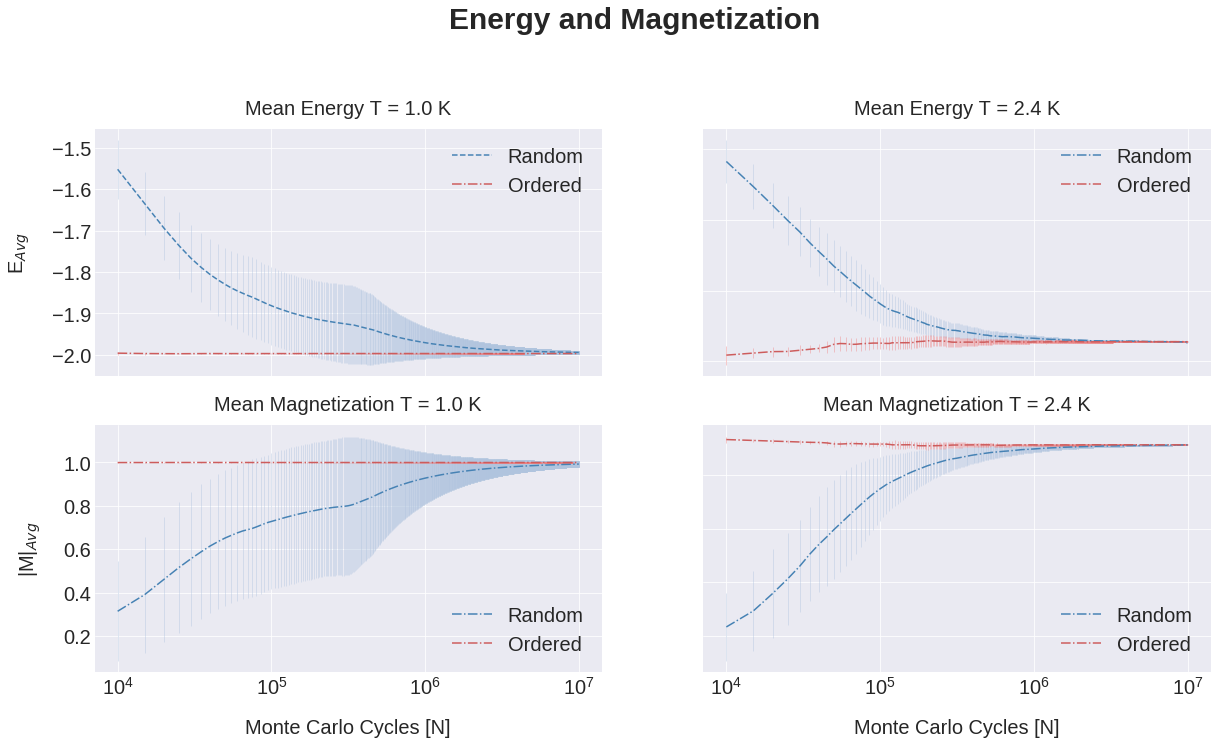
\includegraphics[width = \textwidth]{Figures/4C1.png} 
	\caption{\label{4C11} \textit {The plots show the the expectation value of the energy and absolute value of the Magnetization per spin, as a function of the temperature $T$ and N Monte Carlo iterations. Each point is the sum of the previous $N_i$ points averaged by $N_i$. The system was initiated using both an \textbf{random} and an \textbf{ordered} initial configuration. The ordered configuration was initiated in the ground state with all spins pointing up, the ground state of the system per spin was $\expval{E} = -2$. Thus the equilibration time is much smaller than it is for the random initial configuration. The $\expval{\abs{M}} = 1$ is what one expects when the system has reached equilibrium ground state. The error bars represents the variance of the 10 independent test runs. }}
\end{figure}
\newpage
\vspace{20mm}
\twocolumngrid

     

\newpage 
\begin{figure}[H]
	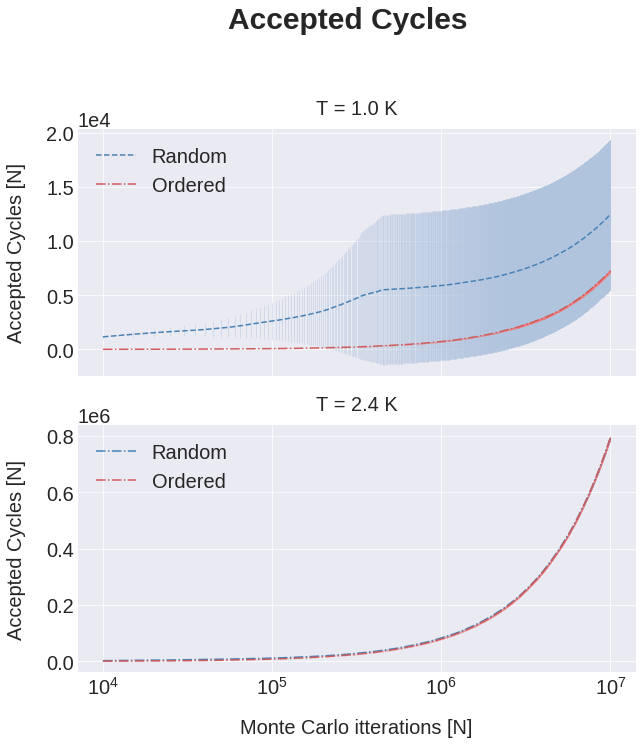
\includegraphics[width = \columnwidth]{Figures/Plot2.png} 
	\caption{\label{4C2} \textit{The number of accepted transitions in the spin configuration as a function of N Monte Carlo iterations, for configurations initiated in both an orderly and random fashion. The error bars represents the variance of 10 independent runs.} \vspace{10mm}
	}
\end{figure} 
\begin{figure}[!h]
	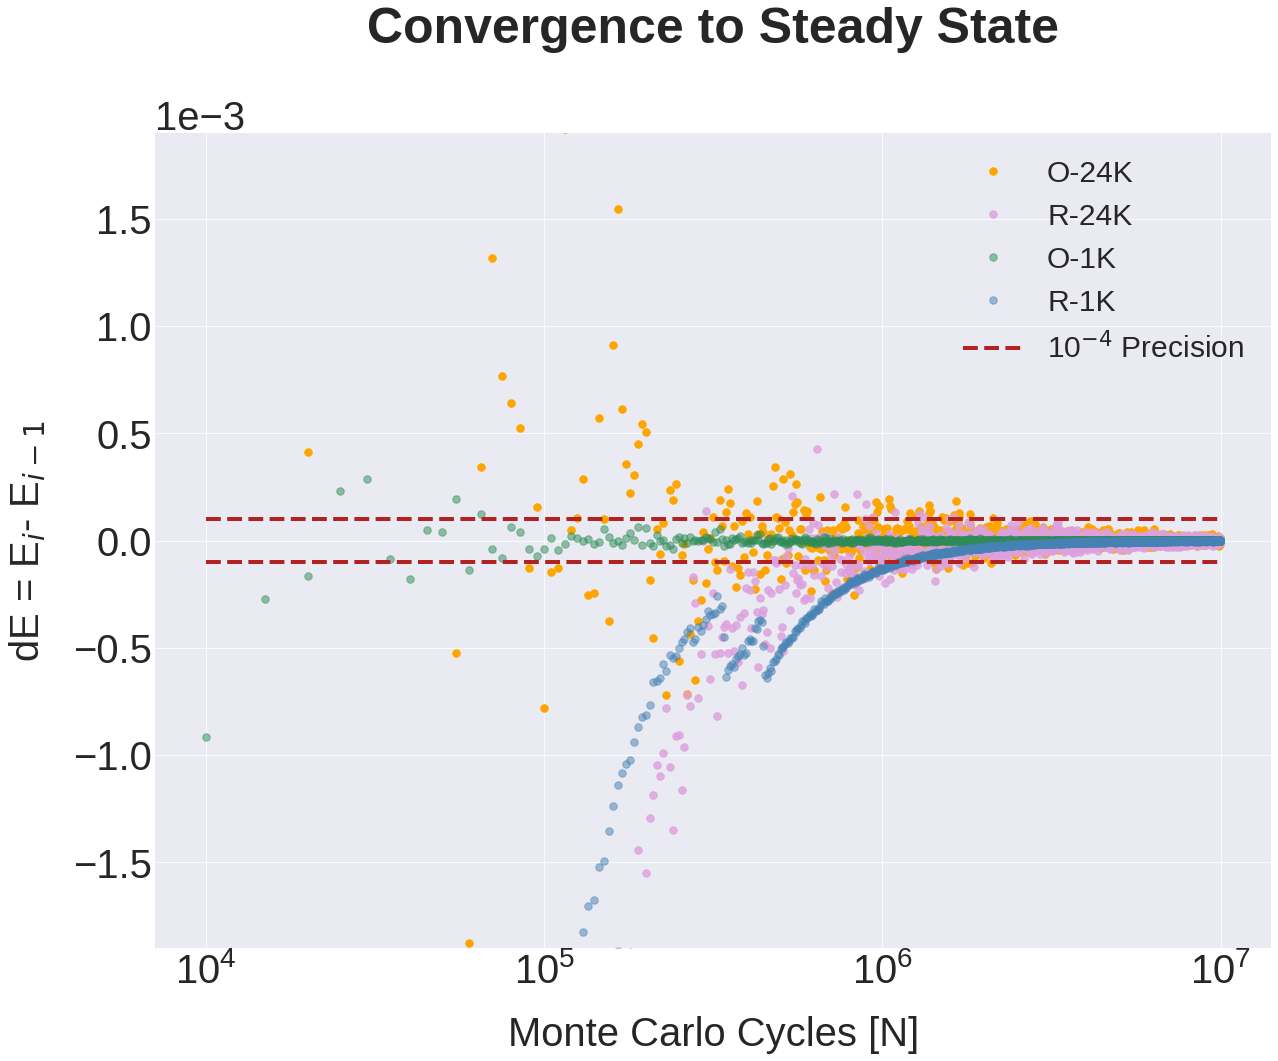
\includegraphics[width = \columnwidth]{Figures/Plot3.png} 
	\caption{\label{4C3} \textit{ The energy difference between two Monte Carlo iterations as function of N. Data is shown for the temperatures $T = 1.0$ $k_bT/J$ and $T = 2.4$ $k_bT/J$, for both random and ordered initial states $S$. The threshold indicated by the red strips is a precision of $10^{-4}$ digits.}}
\end{figure}  

\newpage \noindent 
A graphical evaluation of figure \ref{4C11} shows that the equilibration time in number of Monte Carlo sweeps for $T = 1.0$ $k_bT/J$ is roughly
\begin{equation*}
t_{eq} \approx 2.5\times10^5 \hspace{3mm}[N_{sweeps}]
\end{equation*}\\
while for $T = 2.4$ $k_bT/J$ the equilibration time is roughly \\  
\begin{equation*}
t_{eq} \approx 2.5\times10^4 \hspace{3mm}[N_{sweeps}]
\end{equation*} \\  \indent 
It is evident in figure \ref{4C11} that the curves converge towards $\expval{E} = -1.996$ and the magnetization to $\expval{\abs{M}} = 0.998$. 
The variance of the system initiated with the random initial spin configuration of $S$ indicates large fluctuations in the approximation, while the $S$ matrix initiated with an ordered spin configuration has barely a visible variance. In both cases the variance goes to zero for sufficiently large $N$-values. \\ \indent 
Figure \ref{4C2} shows the number of accepted cycles as a function of the number of Monte Carlo iterations $N$. It is evident that the difference in the number of accepted cycles following an ordered or random initial state are larger for $T = 1.0$ $k_bT/J$ than it is for $T = 2.4$ $k_bT/J$. It is clear that the number of accepted cycles grows exponentially larger faster for $T = 2.4$ $k_bT/J$. \\
Figure \ref{4C3} shows the change in energy for each new configuration $i$, $dE = E_i-E_{i-1}$. The $dE$ becomes zero as $N$ increases, and the equilibrium state is reached. The spread in $dE$ fluctuates more in the case where the evaluation was initiated using a random state, that it was using an ordered state. As well, it is evident that the ordered state has a lower equilibration time than the random initial configuration. \\ \indent   

\subsection*{The probability distribution } \noindent 
Figure \ref{4C4} shows the energy distribution as a function of T. For $T = 1.0$ $k_bT/J$ one can observe two primary bins. The largest selection of $E$ values are found at $E = -800$, while a somewhat smaller fraction is found at $E = - 792$. For $T = 2.4$ $k_bT/J$ it is evidently a broad range of distributed energies present, with a mean of $E = - 700$. The curve enveloping the bins are the fitted curve. The main feature presented in this result, is that more microstates become accessible as the expectation value of the energy increases. 

\onecolumngrid 

\vspace{35mm}
\begin{figure}[H]
	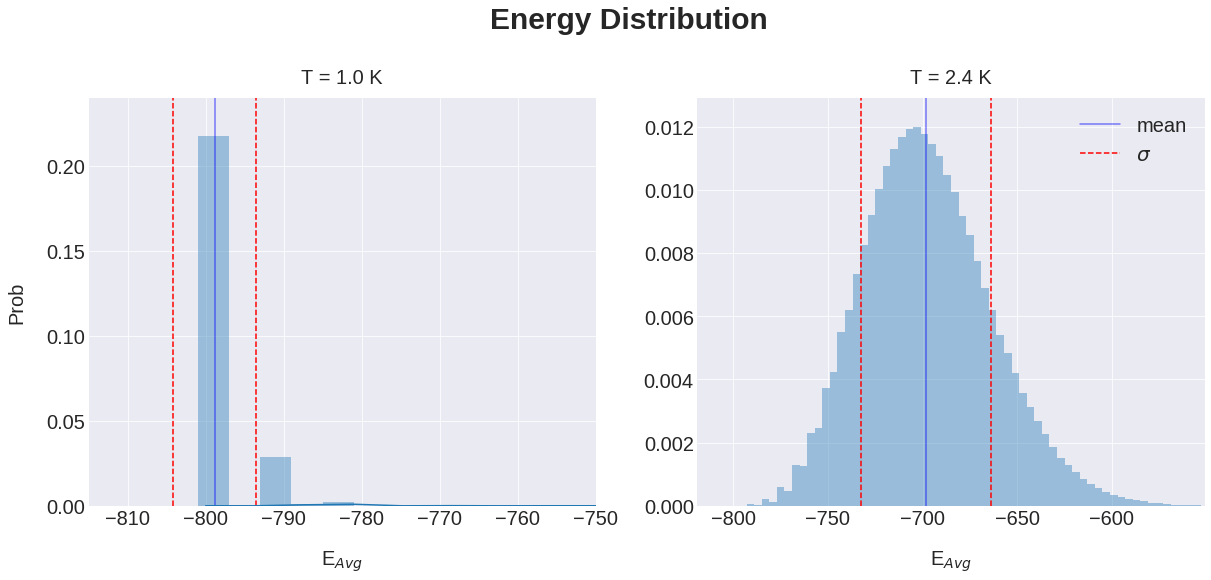
\includegraphics[width = \textwidth]{Figures/Plot4E.png} 
	\caption{ \label{4E} \textit{The energy distributions for $T = 1.0$ $k_bT/J$ and $T = 2.4$ $k_bT/J$, with $L=20$. Each energy count corresponds to one count made in the Monte Carlo iteration procedure that goes into estimating the expectation value, after an initial burn in time of $t_{burn} = 5000L^2$. The lower temperature has primarily two bins at $\bar{E} = -800$ and $E = -992$, with $\bar{E}= -799$ and $\sigma = 5$. The higher temperature has a distribution of energies with $\bar{E}=  -698$ and $\sigma = 34$. The red, stippled lines indicate the standard deviation, and the blue solid line indicates the mean energy.  \vspace{25mm}}}
\end{figure} 

\twocolumngrid \noindent 

\subsection*{Studies of phase transitions} \noindent
Figure \ref{4C5} shows the results of the final experiment which estimate the properties $\expval{E}$, $\expval{\abs{M}}$, $\chi$ and $C_V$ as functions of temperature. Plot of the full temperature range is provided in the appendix, see figure 7. \\ \indent 
For all four values one can see indications of the phase transition in the region around the critical temperature. For the expectation values of the energy, the energy shortly after $T_C$ appears to increase slightly as L increases. \\ \indent
For the expectation value of the magnetization, an increase in $L$ appears to cause the slope of the magnetization curve to decrease faster as the temperature rises. \\ \indent 
The susceptibility $\chi$ illustrates a distribution, who's maximum value appears to be dependent on the value of $L$. $L = 100$ has a maximum closest to the critical temperature $T_C$, while $L = 40$ has the maximum value the furtherest away. \\ \indent 
The same tendency is illustrated in the $C_V$ curves, where an increase in $L$ appears to shift the maximum point towards the critical temperature.  \\ \indent  \newpage 
The maximum values of the interpolated $\chi$ and $C_V$ curves are provided in table \ref{TCc}. The estimates of the critical temperature $T_C$ is provided in table \ref{TCf}, alongside the relative error.
\begin{table}[!h]
	\caption{\label{TCc} The table contains the maximum values found for the $\chi$- and $C_V$ curve of figure \ref{4E}. }
	\begin{tabular}{|c|c|c|} \hline 
		\textbf{L} & $\mathbf{\chi_{max}}$ & $\mathbf{C_{V, max}}$ \\ \hline 
		100 & 2.274 & 2.299\\
		80 & 2.279 & 2.298\\
		60 & 2.282 & 2.304\\
		40 & 2.289 & 2.320\\ \hline 
	\end{tabular}
\end{table}

\begin{table}[!h]
	\caption{\label{TCf} The table contains the maximum values found for the $\chi$- and $C_V$ curve of figure \ref{4E}. }
	\begin{tabular}{|c|c|c|} \hline 
		\textbf{Base} & \textbf{a} & $\mathbf{T_C}$\\ \hline 
		$\mathbf{\chi_{max}}$ & 2.00 & 2.29 $\pm$ 0.01\\
		$\mathbf{C_{V, max}}$   & 0.4 & 2.30 $\pm$ 0.01 \\ 
\hline 
	\end{tabular}
\end{table}
\newpage

\onecolumngrid 

\begin{table}[H]
	\caption{\label{2b}Results per spin of a Metropolis Algorithm using the Ising model on a $2\times 2$ spin-grid. The results are provided as functions of N, for $T = 1.0$ $k_bT/J$. The analytical expectation values are given at the bottom of the table as A.}
	\begin{tabular}{|c|c|c|c|c|c|c|c|} \hline 
		\textbf{N}  & \hspace{1mm}	$\expval{\mathbf{E}}$ \hspace{1mm} & \hspace{1mm}$\expval{\mathbf{E^2}}$ \hspace{1mm} & \hspace{1mm}	$\expval{\mathbf{M}}$\hspace{1mm}  &	\hspace{1mm} $\expval{\mathbf{M^2}}$ \hspace{1mm}  &	\hspace{1mm}$\expval{\abs{\mathbf{M}}} $\hspace{1mm} & \hspace{2mm}$\mathbf{\chi}$	\hspace{2mm} & \hspace{2mm}	\textbf{C}$_V$\hspace{2mm} \\ \hline 
		&&&&&&&\\
		10$^4$   &  -1.9974 $\pm$ 7$\times 10^{-4}$  & 15.979 $\pm$  7$\times 10^{-3}$   &  0.6353 &   3.9958 $\pm$ 6$\times 10^{-4}$&   0.999$\pm$  1$\times 10^{-3}$&   0.0 $\pm$ 4$\times 10^{-1}$&   1.8 $\pm$ 6$\times 10^{-1}$\\
		
		10$^5$    &          -1.9967    $\pm$  4$\times 10^{-4}$    & 15.974   $\pm$  7$\times 10^{-3}$ &  -0.0309 &   3.9946  $\pm$ 3 $\times 10^{-4}$ &   0.9989 $\pm$  9$\times 10^{-4}$&   0.0 $\pm$   2$\times 10^{-1}$ &   3.80 $\pm$  5$\times 10^{-2}$\\ 
		
		10$^6$  &          -1.9958 $\pm $ 1$\times 10^{-4}$   & 15.967   $\pm$   9$\times 10^{-3}$&  -0.0351 &   3.9931 $\pm $ 1$\times 10^{-4}$ &   0.9987 $\pm$  7$\times 10^{-4}$&   0.03  $\pm$   4$\times 10^{-2}$&   3.95 $\pm$   1$\times 10^{-2}$\\ 
		
		10$^7$  &          -1.9960  & 15.968 $\pm$  8$\times 10^{-3}$  &    -0.0037 &   3.9933 &   0.9987 $\pm$ 7$\times 10^{-4}$ &   0.032 $\pm$ $3\times 10^{-3}$&   3.9897 $\pm$ $9\times 10^{-4}$ \\ 
		10$^8$   &          -1.9960 & 15.968 $\pm$ 8$\times 10^{-3}$&  -0.0015 &   3.9933 &   0.9987$\pm$ 7$\times 10^{-4}$&   0.032 $\pm$  $3\times 10^{-3}$   &   3.9931\\ 
		&&&&&&&\\ \hline 
		A &-1.9960 & 16.0926  &0.    &  3.9933 & 0.9980  & 0.0321&  3.9933 \\ \hline 
	\end{tabular}
\end{table} 

\begin{figure}[H]
	\centering 
	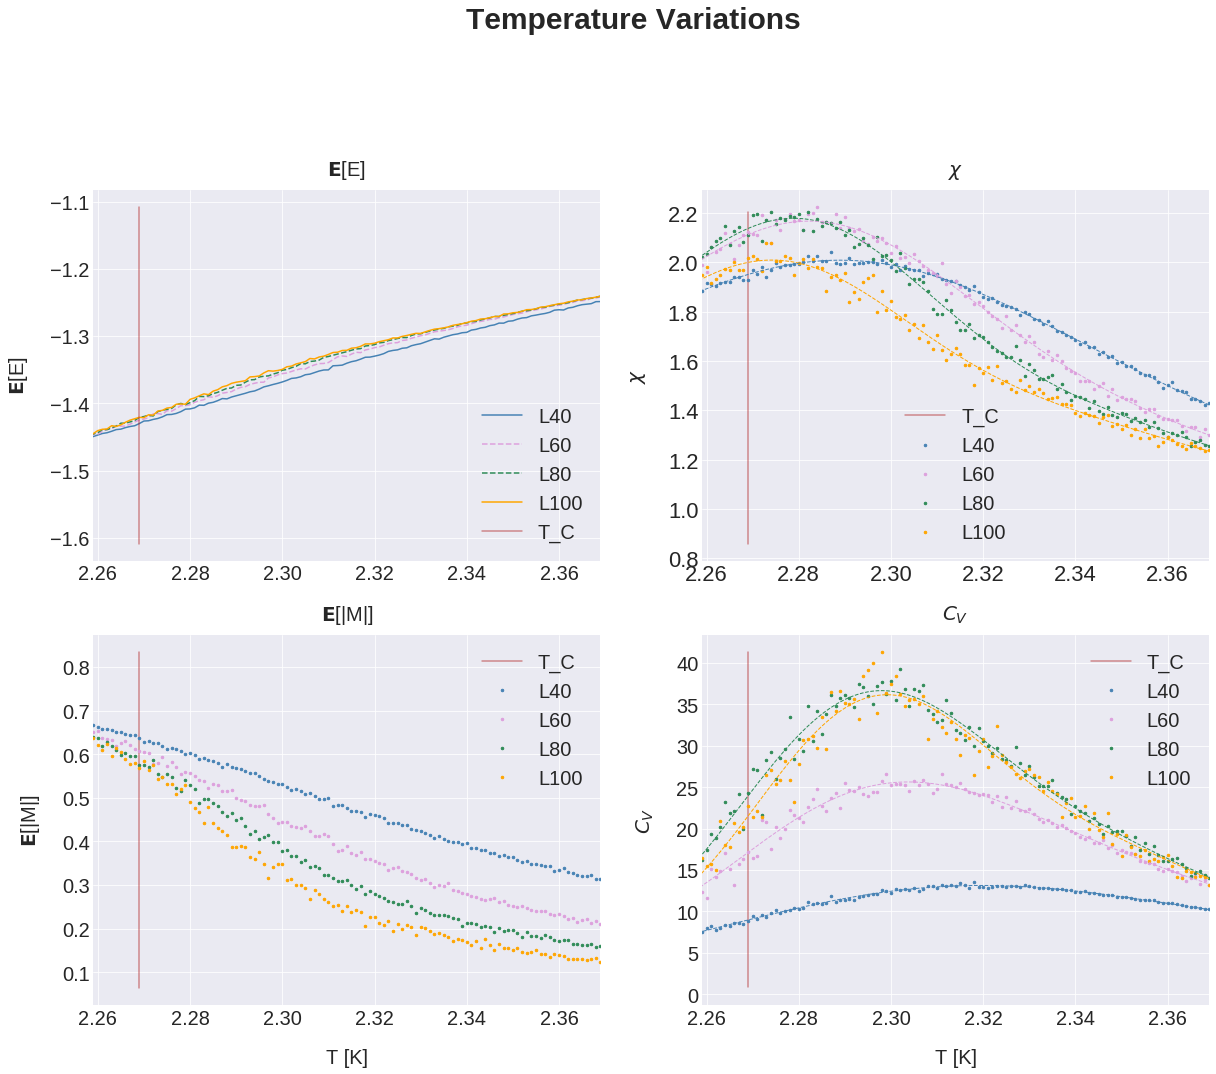
\includegraphics[scale = 0.39]{Figures/plot5.png} 
	\caption{ \label{4C5} \textit{ The figure shows the properties $\expval{E}$, $\expval{\abs{M}}$, $\chi$ and $C_V$ as functions of temperature $T$, which is varied from $T\in[2.15, 2.50]$ with an interval $dT = 10^{-3}$. The system is evaluated for $L \in[40,60,80,100]$, and exhibit tendencies of phase transition around the critical temperature $T_c = 2.269$. All runs were initiated using an ordered spin alignment of all spin up values. The solid lines represent the spline interpolated approximation to the data, represented by the dots. }}
\end{figure} 
\newpage 

\twocolumngrid 


\subsection*{Compilation Time} \noindent 
Table \ref{Compilationtime} presents the time measurement of the parallellized procedure using different compilation flags. The flags $-O2$ and $-O3$ runs significantly faster than using $-O1$ or no flag at all. The runtime also became significantly more unstable with the latter configuration.  
\begin{table}[!h]
	\caption{\textit{The table contains the time estimates of the parallelized procedure, using compiler flag $-O1$, $-O2$ or $-O3$. The results is the mean over 100 measurements, and are presented with the variance of each data set. } \label{Compilationtime}}
	\begin{tabular}{|c|c|} \hline
		\textbf{Compiler Flag}  & \textbf{Time [s]}   \\ \hline
		\textit{-O1} & 23 $\pm$ 9 \\ 
		\textit{-O2} & 11.9 $\pm$ 0.2\\ 
		\textit{-O3} & 11.6 $\pm$ 0.5 \\ 
		\textit{No Flag} &  20 $\pm$ 4\\ \hline 
	\end{tabular}
\end{table}

\section{Discussion} \noindent 
In general, the results found throughout this paper appears to be in good agreement with what is known of Boltzmann statistics and basic thermodynamics. From table \ref{2b} it was apparent that the relative error tended to decreased as $N$ increases, as is expected as the statistical background and convergence rate increases. Although in the case of $\expval{E^2}$, the error tends to stay the same or slightly increase. It should be stated that the error estimates and error propagation techniques applied in this paper are slightly naive. The results would likely benefit a lot from a more through error analysis. This is left for future work.\\  \indent 
Looking towards part two considering the convergence towards an equilibrium state, it was found that the most likely state would be reached faster for a higher T value. That the equilibrium time goes down as the temperature goes up make sense as the probability acceptance rate is proportional to $\Delta E$. The acceptance rate goes up, and therefore more states are excepted. This is also reflected in the distribution graphs presented in figure 4. \\ \indent 
When looking the cycle acceptance rates from figure \ref{4C2}, it is apparent that the functions have more or less the same function form, but that the a higher temperature indicates a more rapid increase in accepted cycles. This makes sense in light of the fact that the $T = 2.4$ $k_bT/J$ have a shorter equilibrium time. When the equilibrium time is reached, almost every cycle will be accepted as $dE = 0$. \\ \indent
In regards to the probability distribution function, it was evident that the mean energy increased as the temperature increased. This is consistent with what we would expect in regards to the theory, where $\expval{E} = \expval{E(\sin(T^{-1}))}$. That is, as the temperature increases more microstates becomes accessible as is consistent with the basics of thermo dynamics. Furthermore, the variance increases as the distribution becomes broader, as it should. The variance also appears to be of an appropriate width when looking directly at the distribution itself. The results therefore appears to be sensible.  \\ \indent
The final results of the critical temperature are decent but have potential for improvement. It is known that the relative error tends to yield an overly optimistic error estimate. This seems to be the case, as the estimate of 1\% do not even include the Onsager estimate of $T_C$.  To evaluate the error in the proper way one would have to include an estimate of the covariance. This is left for future work. It is also clear that a finite grid size of $L = 100$ is quite far from approximating $L\rightarrow\infty$. If more computational power became available, a better solution would be to use a higher value of $L$ to yield a better approximation. This is left for future work as well. 


\section{Conclusion} \noindent 
This paper has considered the evaluation of the Ising model using a Monte Carlo Metropolis approach. Initially a $2\times 2$ grid was employed and compared with the exact values from an analytical evaluation of the system. It was found that $N = 10^7$ Monte Carlo iterations was sufficient to make a good approximation, with an accuracy of minimum three leading digits for all properties. Thereafter the approach was applied to a $20 \times 20$ grid for $T = 1.0$ $k_bT/J$ and $T = 2.4$ $k_bT/J$, and the equilibration time and the number of accepted cycles was considered. The number of accepted cycles were found to increase as T increased. The equilibration time for $T = 1.0$ $k_bT/J$  was found to be $
t_{eq} \approx 2.5\times10^5 \hspace{3mm}[N_{sweeps}]$ and for $T = 2.4$ $k_bT/J$ the equilibration time was set to $t_{eq} \approx 2.5\times10^4 \hspace{3mm}[N_{sweeps}]$. It was again confirmed that both systems had reached equilibrium well within $N = 10^7$ Monte Carlo iterations. \\ \indent 
This paper also investigated the simulation of phase transitions. By varying the grid size $L$, it was possible to produce plots clearly indicating various effects around the region of the critical temperature. That is, varying L yielded differentiating values of the energy expectation value and magnetization expectation value, as well as shifting the maximum values of $\chi$ and $C_V$.  Using this plots to give an estimation of $T_C$ yielded $T_C = 2.29 \pm 0.01$ $k_bT/J$ using $\chi$ and $T_c = 2.30 \pm 0.01$ $k_bT/J$.   \\ \indent 
The final measurements of the run time using various compilation flags showed that there were more or less no difference between using $-O2$ and $-O3$. On the other hand, using no compilation flag at all or $-O1$ tended to increase the run time, and make the run time less stable. \\ \indent 
In the end, the Monte Carlo Metropolis procedure was successful in simulating the Ising model system. It is clear that better approximation could be produced using a larger grid size L or a larger sample of Monte Carlo iterations $N$. This improvements are left for further work. 

\newpage . \newpage

\onecolumngrid 
\section{References} \noindent
[1] L. Onsager, Crystal Statistics. I. A Two-Dimensional Model with an Order-Disorder Transition, Physical Review, 2/1944, Vol.65(3-4), pp.117-149.\\ \noindent
[2] M. Jensen, Lecture Notes in computational physics, 2015 \\ 
\vspace{2cm} \\ 
\noindent 
\textit{Note: The work associated with this paper is avilable from https://github.com/OlineRanum/FYS3150/tree/master/Project\_4}
\newpage
\section{Appendix} \noindent
\subsection{Derivation of thermo-physical quantities for a $2\times 2$ lattice grid} \noindent 
The following section includes the detailed derivation of the $2\times 2$ analytical expectation values used as benchmarked values in this paper. 
\begin{figure}[!h]
	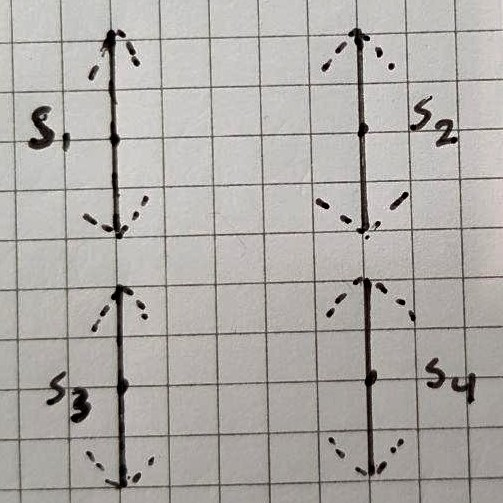
\includegraphics[scale = 0.5]{Figures/si.jpg}
	\caption{\label{si}}
\end{figure}
Each energy state for the various configurations are determined by equation \ref{isemodel}, who for the specific $2\times2$ lattice grid is
\begin{align*}
E_i  =& -J[s_1s_2 + s_1s_3 + s_2s_1+s_2s_4+s_4s_2+s_4s_3 + s_3s_1 + s_3s_4] \nonumber \\
= &-2J[s_1s_2 + s_2s_3 + s_3s_4 + s_4s_1]
\end{align*}\vspace{1mm} 
One can use this relation to estimate the analytical partition function \footnote{By identity: $2\cosh(\alpha) = e^{-\alpha} + e^{\alpha}$}
\begin{align*}
Z = \sum_{i = 1}^{16}e^{2J\beta[s_1s_2 + s_2s_3 + s_3s_4 + s_4s_1]}
=&  2e^{-8J\beta} + 2e^{8J\beta} + 12e^0\nonumber \\
= & 4\cosh(8J\beta) + 12 
\end{align*} 
Using equation \ref{ev} it is evident that the energy expectation value for the system becomes 
\begin{align*}
\expval{E} = -\dfrac{\partial ln Z}{\partial \beta} = -2\dfrac{\partial}{\partial \beta}\ln{[e^{-8J\beta} + e^{8J\beta}]} =& -\dfrac{16J}{Z}[e^{8J\beta} - e^{-8J\beta}] \\ 
& = -\dfrac{32J}{z}\sinh(8J\beta)
\end{align*}
Table \ref{bc} shows all configurations and their corresponding energy $E_i$ and magnetization $M_i$

\begin{table}[!h]
	\caption{\label{bc} The 16 configurations for a $2\times 2$ Ising model on a 2D lattice. The energy $E_i$ and magnetization $M_i$ for each configuration $i$ is provided.}
	\begin{tabular}{|c|c|c|c|} \hline 
		S$_i$&S$_\uparrow$ & \textbf{$E_i$} [J]&$ M_i$ [\#] \\ \hline   
		0& $\uparrow\uparrow\uparrow\uparrow$ &-8J&4\\
		1&$\uparrow\uparrow\uparrow\downarrow$ & 0&2\\
		2&$\uparrow\uparrow\downarrow\uparrow$ &0&2\\
		3&$\uparrow\downarrow\uparrow\uparrow$ &0&2\\
		4&$\downarrow\uparrow\uparrow\uparrow$ &0&2\\
		5&$\uparrow\uparrow\downarrow\downarrow$ &0&0\\
		6&$\downarrow\downarrow\uparrow\uparrow$ &0&0\\
		7&$\uparrow\downarrow\uparrow\downarrow$ &0&0\\
		8&$\downarrow\uparrow\downarrow\uparrow$ &0&0\\
		9&$\downarrow\uparrow\uparrow\downarrow$ &8J&0\\
		10&$\uparrow\downarrow\downarrow\uparrow$ &8J&0\\
		11&$\uparrow\downarrow\downarrow\downarrow$ &0&-2\\
		12&$\downarrow\uparrow\downarrow\downarrow$ &0&-2\\
		13&$\downarrow\downarrow\uparrow\downarrow$ &0&-2\\
		14&$\downarrow\downarrow\downarrow\uparrow$ &0&-2\\
		15&$\downarrow\downarrow\downarrow\downarrow$ &-8J&-4\\\hline 
	\end{tabular}
\end{table}


The specific heat capacity of this system can be calculated using equation $cv$, 
\begin{align}
\expval{E^2} = \dfrac{1}{Z}\sum_{i=1}^{16}E_ie^{-\beta E_i}  = & \dfrac{128J^2}{Z}(e^{8J\beta} + e^{-8J\beta}) \\
=& \dfrac{258J^2}{Z}\cosh(8J\beta)
\end{align}
It follows that 
\begin{align}
C_V =& \dfrac{\beta}{T}\qty[\dfrac{258J^2\cosh(8J\beta)}{4\cosh(8J\beta) + 12 }  -\qty(-\dfrac{32J\sinh(8J\beta)}{4\cosh(8J\beta) + 12 })^2] \nonumber \\
= & \dfrac{\beta}{T}64J^2\qty[\dfrac{\cosh(8J\beta)}{\cosh(8J\beta) + 3}  -\qty(\dfrac{\sinh(8J\beta)}{\cosh(8J\beta) + 3 })^2]\nonumber \\ \nonumber & \\ & 
\end{align}
The mean magnetization becomes 
\begin{align*}
\expval{M} =& \dfrac{1}{Z}\sum_{i = 1}^{16} M_ie^{-\beta E_i} \\ 
= & \dfrac{1}{Z}\qty(4e^{8J\beta} +4\times 2e^0 + 4\times(-2)e^0 -4e^{8J\beta}) \\
= & 0
\end{align*}
\begin{align*}
\expval{\abs{M}} =& \dfrac{1}{Z}\sum_{i = 1}^{16} \abs{M_i}e^{-\beta E_i} \\ 
= & \dfrac{1}{Z}\qty(4e^{8J\beta} +4\times 2e^0 + 4\times2e^0 +4e^{8J\beta}) \\
= & \dfrac{8e^{8J\beta}}{4\cosh(8J\beta) + 12 } \\
= & \dfrac{2e^{8J\beta}}{\cosh(8J\beta) + 3 }
\end{align*}
\begin{align*}
\expval{M^2} =& \dfrac{1}{Z}\sum_{i = 1}^{16} M_i^2e^{-\beta E_i} \\ 
= & \dfrac{1}{Z}\qty(16e^{8J\beta} +4\times 4e^0 + 4\times4e^0 + 16e^{8J\beta}) \\
= & \dfrac{8e^{8J\beta} + 8}{\cosh(8J\beta) + 3}
\end{align*}
Yielding the susceptibility 
\begin{align}
\chi =& \dfrac{\beta}{T}\qty(\expval{M^2}- \expval{M}^2)\\
=& \dfrac{\beta}{T}\dfrac{8e^{8J\beta} + 8}{\cosh(8J\beta) + 3}
\end{align}
\newpage

\subsection{Full scale plots of phase transitions}
Figure \ref{4C4} includes the full scale plots of the data used to evaluate phase-transitions in this paper. 
\begin{figure}[H]
	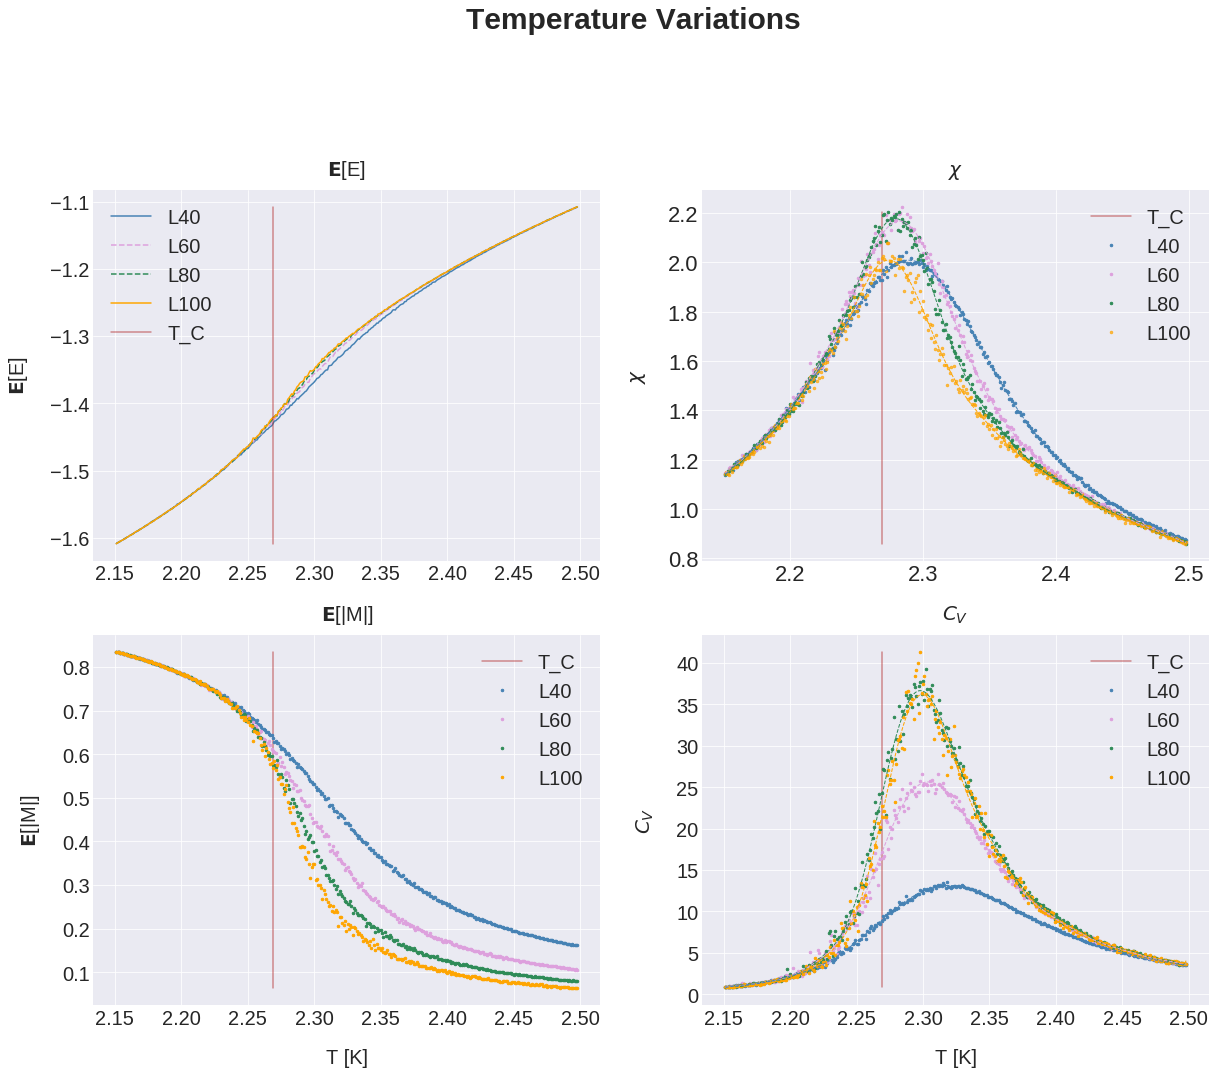
\includegraphics[width = \textwidth]{Figures/plot4.png} 
	\caption{ \label{4C4} The energy distributions for $T = 1.0$ $k_bT/J$ and $T = 2.4$ $k_bT/J$, with $L=20$. The lower temperature has primarily two bins at $\bar{E} = -800$ and $E = -992$, with $\bar{E}= -799$ and $\sigma = 5$. The higher temperature has a distribution of energies with $\bar{E}=  -698$ and $\sigma = 34$. \vspace{10mm}}
\end{figure} 

 
\end{document}